\documentclass[12pt]{report}

\usepackage{amsmath}
\usepackage{graphicx}
\usepackage[a4paper,left = 40pt, right = 40pt, top = 80pt, bottom = 100pt]{geometry}

\begin{document}
\author{Mohit, 20d070052 }
\title{ EE324 : Controls Lab \\ Lab 3 Report \\Noise cancellation in headphones\\Group 16}
\maketitle

\newpage

\begin{Large}
Aim:\\

To design and implement an analog circuit for noise cancellation in

headphones. using the IR sensors provided on the robot for this purpose.\\

\vspace{15pt}

\begin{Large}
Objectives:\\
\end{Large}
\begin{enumerate}
    \item To achieve an attenuation of 20 dB, when a noise of 100 Hz frequency is applied.
    \item To design an analog compensator to stabilize the system, i.e. loop shaping of the loop
transfer function.\\
\end{enumerate}

\\


\vspace{15pt}

\begin{Large}
Prerequisites:\\
\end{Large}

System identification (frequency response analysis), Compensator design 

and implementation,Matlab coding.\\

\vspace{15pt}

\begin{Large}

Equipment used:\\
\end{Large}


Headphone setup, DSO, Function generator, Probes, Amplifier ICs,

Breadboard, Wires,Jumpers,Wire stripper.\\

\newpage
\begin{Large}
Methods:\\
\end{Large}


Procedure:\\

\begin{Large}
\begin{itemize}
 
    
\item Applied sinusoidal input to the Headphone setup using function generator and calculated peak-peak voltage of input and output using DSO.

\item The gain of the Headphone setup is calculated by dividing peak-to-peak voltages of input and output is used to plot frequency response(magnitude and phase plot) of the Headphone setup .

\item After studying the magnitude and phase response of the Headphone setup we tried to achieve an attenuation of 20 dB, when a noise of 100 Hz frequency is applied to the input in MATLAB

\item After above constrained is achieved we designed lag compensator to stablize the system.

\item The poles and zeros of the lag compensator were tuned to make the negative gain margin magnitude greater than 3 dB phase margin magnitude greater than 30 degrees.
\vspace{3em}
\end{itemize}

\end{Large}
\begin{Large}
Observations:\\
\end{Large}

We observe that our setup is successful achieveing the required constrain

of the LAB of attenuation of 20 dB, when a noise of 100 Hz frequency is

applied ,and system is stable after implementing the compensator to it.\\

\newpage
\begin{Large}
Problems Faced: \\
\end{Large}

\begin{itemize}
\item It was difficult to get the readings for frequency response in a noisy
surrounding .
\item Reading of Peak-peak voltage and phase difference was fluctuating in DSO.
 Due to which got wrong readings.

\item Hard to find values of resistances and capacitance which were available for designing the compensator .
\end{itemize} 

\vspace{20pt}
\begin{Large}
Parameters Obteined: \\
\end{Large}
\begin{itemize}
    \item Transfer function of Compensator = 
    \item Gain Margin = 
    \item Phase margin = 
    \item Gain at 100Hz = 
\end{itemize}

\newpage
\begin{Large}
Experiment Completion Status:\\
\end{Large}

The experiment has been completed .\\

\begin{figure}[h!]
\center
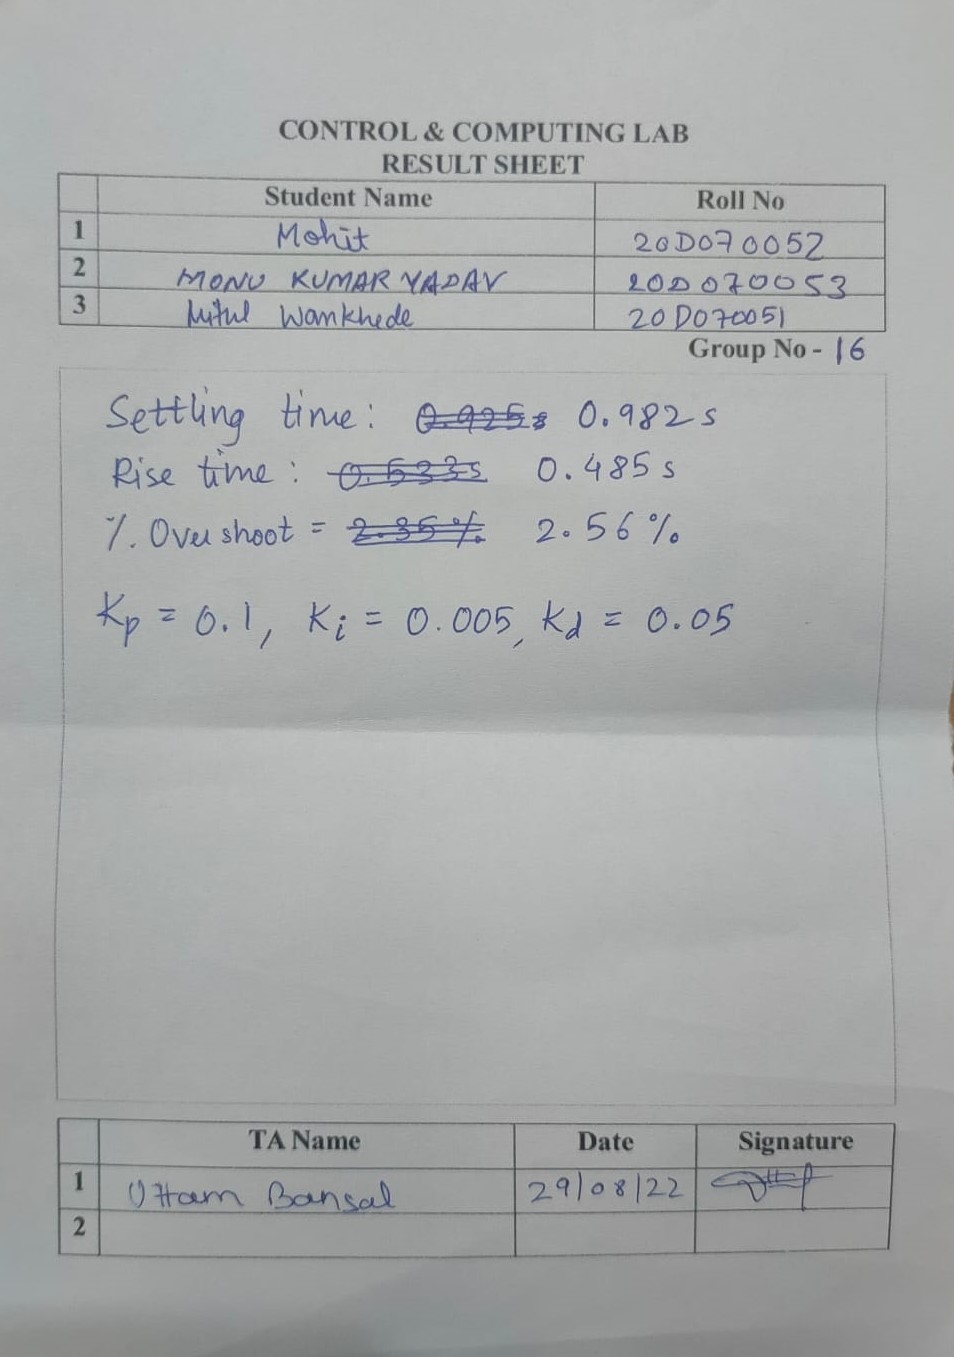
\includegraphics[width=310pt]{Result.jpeg}
\end{figure}



\end{document}
